\chapter{The Transport Equation}

In this lecture, we introduce general \textit{transport equations} and finish by developing the form used in neutron transport theory.  In the lectures to follow, we shall describe other aspects of the neutron transport equation and methods by which it can be solved both analytically and numerically.

\section*{Transport Theory}

Transport theory aims to describe mathematically the movement (i.e. ``transport'') of particles as they traverse a medium.  For example, we might describe the transport of high energy gammas through a lead shield, or the movement of neutrons through uranium dioxide pellets.  We might also describe the movement of particles in a dense gas as they navigate through a medium consisting of the gas itself.

In all cases, transport theory describes such processes in an \textit{average} sense.  For instance, we do not compute the individual trajectories of neutrons in a reactor via transport theory.  That, instead, would require molecular dynamics, in which Newton's equation of force is solved for the many-bodied problem of all neutrons in the vicinity of interest (an essentially impossible problem), or perhaps the Monte Carlo methods described in previous lectures, where a sample of individual particles are tracked to approximate ensemble averages (a difficult, but as we've seen, tractable problem).  Hence, the quantities we shall compute using the equations of transport theory should be recognized as expected and not exact values.

\section*{Fundamental Quantities}

We begin by defining several fundamental quantities.  It should be noted that the forms introduced at first are likely different from what you might have seen in a previous reactor physics course.  The purpose here is two-fold.  First, we wish to introduce the quantities and eventually the equations in a general way to make clear that transport theory is not restricted to the neutron transport equation.  Second, for those who might be familiar with, e.g., the Boltzmann equation of gas dynamics (and not neutron transport), the notation will be familiar and lead smoothly into our more familiar form.

We first define the \textit{phase space density function}, the knowledge of which we can use to compute essentially all quantities of interest:
\begin{center}
  \begin{tabular}{cp{7.0cm}}
    $n(\mathbf{r},\mathbf{v},t)d^3r d^3v \equiv $ &
    expected number of particles in  $d^3r$  about  $\mathbf{r}$  with velocity  $dv$ about  $\mathbf{v}$ at time $t$.  
  \end{tabular}
\end{center}
It is often most convenient to break the velocity into its scalar (speed) and vector (direction) components.  The scalar component is recast in the energy variable via $E = mv^2/2$, and the direction vector is defined $\mathbf{\Omega}=\mathbf{v}/|\mathbf{v}|$.  The phase space density can then be rewritten as
\begin{center}
  \begin{tabular}{cp{7.0cm}}
    $n(\mathbf{r},\mathbf{\Omega},E,t)d^3r d\Omega dE \equiv $ &
    expected number of particles in  $d^3r$  about  $\mathbf{r}$  going in the directions $d\Omega$ about $\mathbf{\Omega}$ with energy  $dE$ about  $E$ at time $t$.  
  \end{tabular}
\end{center}
In this form, $n(\mathbf{r},\mathbf{\Omega},E,t)$ is often referred to as the angular density.

\begin{wrapfigure}{r}{0.5\textwidth}
    \begin{center}
    \includegraphics[keepaspectratio, width = 2.7 in]{images/phase_space}
    \end{center}
    \caption{Schematic of Phase Space.}
    \label{fig:phase_space}
\end{wrapfigure}

We can relate the phase space densities in terms of $\mathbf{v}$ and $(E,\mathbf{\Omega})$ via the relations
\begin{equation}
 \begin{split}
  n(\mathbf{r},E,\mathbf{\Omega},t) &= (v/m) n(\mathbf{r},\mathbf{v},t) \\
  n(\mathbf{r},E,\mathbf{\Omega},t) &= (1/mv) n(\mathbf{r},v,\mathbf{\Omega},t) \\
  n(\mathbf{r},v,\mathbf{\Omega},t) &= v^2 n(\mathbf{r},\mathbf{v},t) \, ,
 \end{split}
 \label{eq:densityrelations}
\end{equation}
proofs of which are left as exercises.

Figure \ref{fig:phase_space} depicts a schematic of the phase space used in terms of the position $\mathbf{r}$ and direction $\mathbf{\Omega}$.  The position vector is further broken down into the polar angle $\theta$ and azimuthal angle $\phi$.  The differential solid angle element $d\Omega$ is also shown, and can be expressed in terms of $\theta$ and $\phi$ via
\begin{equation*}
 d\Omega = \sin{\theta} d\theta d\phi \, .
\end{equation*}  
%One might envision such solid angle elements as the small bumps on basketballs.  

A quantity closely related to the phase space density (or current density) is the \textit{angular current density}:
\begin{center}
  \begin{tabular}{cp{5.0cm}}
    $\mathbf{j}(\mathbf{r},\mathbf{v},t)\cdot d\mathbf{S} d^3v = \mathbf{v} n(\mathbf{r},\mathbf{v},t) \cdot d\mathbf{S} d^3v \equiv $ &
    expected number of particles that cross an area $dS$ per second with velocity $d^3v$ about $\mathbf{v}$ at time $t$.
  \end{tabular}
\end{center}

We can also define \textit{partial currents} with respect to a particular surface $S$ defined by an outward normal vector $\mathbf{\hat{e}}_s$:

\begin{center}
  \begin{tabular}{cp{5.0cm}}
    $J_{\pm}(\mathbf{r},t) = \pm \int_{\pm} d^3v  \mathbf{\hat{e}}_s \cdot \mathbf{j} (\mathbf{r},\mathbf{v},t) \equiv $ &
   the rate at which particles flow through $S$ in the outward (+) or inward (-) direction.
  \end{tabular}
\end{center}

The \textit{current density} $\mathbf{J}(\mathbf{r},t)$ is defined by integrating the angular current density over all velocities.  Then for our surface $S$, the net rate of particles passing outward through $S$ is just $\mathbf{J}(\mathbf{r},t) \cdot \mathbf{\hat{e}}_s$.  From our definition of partial currents, the net current passing outward must also be $J_+ - J_-$, yielding the useful identity
\begin{equation}
 \mathbf{J}(\mathbf{r},t) \cdot \mathbf{\hat{e}}_s = J_{+}(\mathbf{r},t) - J_{-}(\mathbf{r},t) \, .
 \label{eq:net2partial}
\end{equation}

%A point of caution: it should be noted that $n$ and $\mathbf{j}$ must have the same units but represent wholly different things since $n$ is a scalar quantity while $\mathbf{j}$ is a vector quantity.  This will be true also of $\mathbf{J}$ and the scalar flux $\phi$, which will be introduced

Of particular interest to us in the next section will be reaction rates, which can most easily be described using the \textit{angular flux}
\begin{center}
  \begin{tabular}{cp{2.0cm}}
    $ \psi (\mathbf{r},\mathbf{\Omega},E,t) = v n(\mathbf{r},\mathbf{\Omega},E,t) \equiv $ &
    angular flux
  \end{tabular}
\end{center}
and \textit{scalar flux}
\begin{center}
  \begin{tabular}{cp{2.0cm}}
    $ \phi (\mathbf{r},E,t) = \int_{4\pi} d\Omega \psi (\mathbf{r},\mathbf{\Omega},E,t)  \equiv $ &
    scalar flux.
  \end{tabular}
\end{center}

\section*{A General Transport Equation}

Consider an arbitrary volume $V$ with a surface $S$.  Our goal is to represent the time rate of change of the particle density $n(\mathbf{r},\mathbf{v},t)$ within the volume.  Neglecting external forces, the only factors affecting the density are collisions within the volume that change a particle's velocity, the streaming of particles into and out of the surface, and any internal source of particles.  This simple balance can be expressed mathematically as
\begin{equation}
\begin{split}
 \overbrace{ \frac{\partial}{\partial t} \Bigg ( \int_V d^3 r n(\mathbf{r},\mathbf{v},t) \Bigg ) }^{\text{total rate of change of }n\text{ in } V} 
      &=  - \overbrace{\int_S dS \mathbf{\hat{e}}_S \cdot \mathbf{j}(\mathbf{r},\mathbf{v},t) }^{\text{streaming rate}}
       + \overbrace{ \int_V d^3 r \Big( \frac{\partial n}{\partial t} \Big )_{\mathrm{coll}} }^{\text{collision rate}} \\
      &+ \underbrace{ \int_V d^3 r s(\mathbf{r},\mathbf{v},t) }_{\text{source emission rate}}  \, ,
\end{split}
\label{eq:balance}
\end{equation}
where $s$ represents a source inside the volume and $(\partial n/\partial t)_{\mathrm{coll}}$ is the time rate of change due to collisions, specific forms of which are application-dependent and will be discussed below.  Note the minus sign on the surface integral, i.e., the streaming term.  Since the integral describes the net rate of neutrons going \textit{out} of the surface, we negate it so that a positive net rate directed inward is a positive contribution to the total time rate of change of $n$ in $V$.

\EQ{eq:balance} gives us a simple relation in terms of both volume and surface integrals.  Our life is always easiest if we have the same integration on both sides.  By the divergence (or Gauss') theorem, we can rewrite the streaming term
\begin{equation}
 \int_S dS \mathbf{\hat{e}}_S \cdot \mathbf{j}(\mathbf{r},\mathbf{v},t) = \int_V d^3r \nabla \cdot \mathbf{j}(\mathbf{r},\mathbf{v},t) \, .
\end{equation}
Because $\nabla$ acts on $\mathbf{r}$ and not $\mathbf{v}$, we note $ \nabla \cdot \mathbf{j} = \nabla \cdot (\mathbf{v} n) =  \mathbf{v} \cdot \nabla n + \overbrace{ n \nabla \cdot \mathbf{v}}^{\to 0} = \mathbf{v} \cdot \nabla n$.  Hence, the streaming term becomes
\begin{equation}
 \int_V d^3r \nabla \cdot \mathbf{j}(\mathbf{r},\mathbf{v},t) = \int_V d^3r \mathbf{v} \cdot \nabla n(\mathbf{r},\mathbf{v},t) \, .
\end{equation}

For a constant volume, $(\partial/\partial t) \int_V d^3 r n = \int_V d^3 r (\partial n/\partial t)$, and so our balance equation can be rewritten as
\begin{equation}
\begin{split}
 \overbrace{  \Bigg ( \int_V d^3 r \frac{\partial}{\partial t}n(\mathbf{r},\mathbf{v},t) \Bigg ) }^{\text{total rate of change of }n\text{ in } V} 
      &=  - \overbrace{\int_V d^3r \mathbf{v} \cdot \nabla n(\mathbf{r},\mathbf{v},t)}^{\text{streaming rate}}
       + \overbrace{ \int_V d^3 r \Big( \frac{\partial n}{\partial t} \Big )_{\mathrm{coll}} }^{\text{collision rate}} \\
      &+ \underbrace{ \int_V d^3 r s(\mathbf{r},\mathbf{v},t) }_{\text{source emission rate}}  \, .
\end{split}
\label{eq:balance2}
\end{equation}
For an arbitrary volume $V$, the integrands of \EQ{eq:balance2} must vanish, yielding a general transport equation:
\begin{equation}
  \frac{\partial}{\partial t}n(\mathbf{r},\mathbf{v},t) = -\mathbf{v} \cdot \nabla n(\mathbf{r},\mathbf{v},t) + \Big( \frac{\partial n}{\partial t} \Big )_{\mathrm{coll}} +  s(\mathbf{r},\mathbf{v},t) \, .
\end{equation}

\section*{Even More Generality}
We can skip the differential volume formulation by considering the material derivative of $n$ (using Cartesian coordinates):
\begin{equation}
 \begin{split}
 \frac{Dn}{Dt} &\equiv \frac{ \partial n}{\partial t} 
 + \frac{\partial x}{\partial t}\frac{\partial n}{\partial x} + \frac{\partial y}{\partial t}\frac{\partial n}{\partial y} + \frac{\partial z}{\partial t}\frac{\partial n}{\partial z} +  \frac{\partial v_x}{\partial t}\frac{\partial n}{\partial v_x} +  \frac{\partial v_y}{\partial t}\frac{\partial n}{\partial v_y} +  \frac{\partial v_z}{\partial t}\frac{\partial n}{\partial v_z} \\
               &= \frac{ \partial n}{\partial t} + \mathbf{v}\cdot \nabla n + \mathbf{a} \cdot \nabla_{\mathbf{v}} n \\
               &= \frac{ \partial n}{\partial t} + \mathbf{v}\cdot \nabla n + \frac{\mathbf{F}}{m} \cdot \nabla_{\mathbf{v}} n \, ,\\
 \end{split}
\end{equation}
where $\nabla_{\mathbf{v}}$ is the gradient operator with respect to velocity components (rather than spatial coordinates).  The material derivative is the total time rate of change, accounting for convective (streaming) effects as well as the influence of an external force $\mathbf{F}$, a factor we did not account for above.  

This total rate of change must be balanced by sources and sinks, which are the collision and internal source terms.  Hence, an even more general transport equation can be written
\begin{equation}
  \frac{\partial n}{\partial t} + \mathbf{v} \cdot \nabla n + \frac{\mathbf{F}}{m} \cdot \nabla_{\mathbf{v}} n =   \Big( \frac{\partial n}{\partial t} \Big )_{\mathrm{coll}} +  s \, .
 \label{eq:generalte}
\end{equation}

\section*{Neutron Transport}

To arrive at the neutron transport equation, we bring back the macroscopic cross-sections studied in Lecture \ref{lec:macro}.  Using our definition for the angular flux, the volumetric collision rate at a particular point in phase space and time is simply
\begin{equation}
 R_{\text{coll}}(\mathbf{r},\mathbf{\Omega},E,t) = \psi(\mathbf{r},\mathbf{\Omega},E,t) \Sigma_t(\mathbf{r},E) \, .
\end{equation}
However, we know that neutrons at one energy and angle can scatter into another energy and angle, and so in general, the rate at which neutrons at any angle and energy are scattered into a particular energy and angle is
\begin{equation}
 R_{\text{in-scatter}}(\mathbf{r},\mathbf{\Omega},E,t) = \int^{\infty}_{0} dE' \int_{4\pi} d\Omega' \Sigma_s(\mathbf{r},\mathbf{\Omega}\cdot\mathbf{\Omega}',E'\to E)\psi(\mathbf{r},\mathbf{\Omega'},E',t) \, .
\end{equation}
The time rate of change due to collisions is thus
\begin{equation}
\begin{split}
 \Big( \frac{\partial n}{\partial t} \Big )_{\mathrm{coll}} &= -\psi(\mathbf{r},\mathbf{\Omega},E,t) \Sigma_t(\mathbf{r},E)  \\
  &+ \int^{\infty}_{0} dE' \int_{4\pi} d\Omega' \Sigma_s(\mathbf{r},\mathbf{\Omega}'\to \mathbf{\Omega},E'\to E)\psi(\mathbf{r},\mathbf{\Omega'},E',t) \, .
\end{split}
\end{equation}
Substituting this into the general transport equation, using $\psi = vn$, and neglecting any external forces, we find the neutron transport equation:
\begin{equation}
  \begin{split}
     \frac{1}{v}\frac{\partial \psi}{\partial t} &+ \hat{\Omega} \cdot \nabla \psi + \Sigma_t \psi(\mathbf{r},\mathbf{\Omega},E,t) = \\
           &+ \int^{\infty}_{0} dE' \int_{4\pi} d\Omega' \Sigma_s(\mathbf{r},\mathbf{\Omega}\cdot\mathbf{\Omega}',E'\to E)\psi(\mathbf{r},\mathbf{\Omega'},E',t) +s \, .
  \end{split}
  \label{eq:neutrontransport}
\end{equation}
Note, the source term $s$ has been used to represent internal sources but could also account for other sources such as fission (though the specific form is, of course, hidden).

\section*{Assumptions for the Neutron Transport Equation}
In writing down Eq. \ref{eq:neutrontransport} as we have, a number of assumptions have been made explicitly or implicitly.  These include:
\begin{enumerate}
   \item The neutron density is large so that it makes sense to be computing for mean values (which is all transport equations can provide)
   \item The neutrons are point particles, meaning that wave effects are insignificant
   \item Collisions are well-defined, two-body interactions that occur instantaneously (delayed neutrons from fission, which are not covered here, are a notable exception and deserve special treatment)
   \item Between collisions, neutrons stream with a constant velocity
   \item Neutron-neutron interactions are negligible
   \item The properties of the medium are assumed known and time-independent (burnup in a reactor is another exception)
   \item The medium is taken to be isotropic (i.e. no directional-dependence)
\end{enumerate}

% 
% \section*{Boundary and Initial Condtions}
% 
% In the last lacture, we finished with the Eq. \ref{eq:neutrontransport} neutron transport equation:
% \begin{equation*}
%   \begin{split}
%      \frac{1}{v}\frac{\partial \psi}{\partial t} &+ \hat{\Omega} \cdot \nabla \psi + \Sigma_t \psi(\mathbf{r},\mathbf{\Omega},E,t) = \\
%            &+ \int^{\infty}_{0} dE' \int_{4\pi} d\Omega' \Sigma_s(\mathbf{r},\mathbf{\Omega}\cdot\mathbf{\Omega}',E'\to E)\psi(\mathbf{r},\mathbf{\Omega'},E',t) +s \, .
%   \end{split}
% \end{equation*}

\subsection*{Initial Conditions}

This is an integro-differential equation in 7 variables: 3 in space, 2 in angle, 1 in energy, and time.  Like all differential equations, the transport equation requires initial and boundary conditions. 


Initial conditions for the transport equation are relatively straightforward.  At some initial time $t_0$, an initial condition is expressed as
\begin{equation}
 \psi(\mathbf{r},\mathbf{\Omega},E,t)|_{t=t_0} = f(\mathbf{r},\mathbf{\Omega},E) \, ,
\end{equation}
where $f$ represents a known function of space, angle, and energy.  

Time-dependent problems in neutron transport are often quite challenging due to the wide range of time scales involved.  A good example comes from the study of reactor kinetics, where the time scales range from prompt neutron lifetimes (on the order of 10$^{-5}$ seconds) to the delayed neutrons of longest lifetime (on the order of tens of seconds).  Any numerical scheme is effectively limited by the smallest time scale, leading to a ``stiff'' problem.  

Other neutron transport problems exhibit even more diverse time scales.  The time scale for nuclear weapons is perhaps most easily quantified with ``shakes'', that is 10$^{-8}$ seconds.  Isotopic changes in nuclear reactors due to irradiation can have profound effects on time scales ranging from hours (xenon production) up to months or years (burnup).

Frequently, we are interested in steady state values, so that $\frac{\partial \psi}{\partial t} = 0$.  If the source $s$ in Eq. \ref{eq:neutrontransport} includes an external source, then the problem is a \textit{fixed source problem}.  If $s$ does not include an external source (and includes only e.g. a fission source), then the problem becomes an \textit{eigenvalue problem}, which are studied in Lecture \ref{lec:criticality}.

\subsection*{Boundary Conditions}

The most straightforward boundary condition to enforce is the \textit{free surface} or \textit{vacuum} condition.  Physically, the condition represents the situation where no neutrons enter a volume from the outside.  In other words, the volume of interest can be thought to exist in a void.  Mathematically, the condition is expressed
\begin{equation}
 \psi(\mathbf{r},\mathbf{\Omega},E,t) = 0 \, , \, \, \, \,  \, \, \, \mathbf{\hat{n}} \cdot \mathbf{\Omega} < 0 \, ,
\end{equation}
where $\mathbf{\hat{n}}$ is the unit \textit{outward normal} vector to the surface of interest.  
% is there a better way to give nice wrapping??  
\begin{wrapfigure}{r}{0.3\textwidth}
    \begin{center}
    \includegraphics[keepaspectratio, width = 1.25 in]{images/squarecylinder}
    \end{center}
    \caption{A reentrant square cyclinder.}
    \label{fig:squarecylinder}
\end{wrapfigure}
Since $\mathbf{\hat{n}} \cdot \mathbf{\Omega}$ is just the cosine of the angle between the incident neutrons and the normal vector, we see the flux vanishes whenever that cosine is negative, or whenever the neutron direction is inward.

A point of warning: reentrant geometries must be avoided when using vacuum conditions.  Unless treated with special care, reentrant geometries lead to inconsistency.  Neutrons leaving one portion of the geometry could, in theory, reenter another portion, but since vacuum conditions disallow this, the true problem is not modeled correctly.  A common example of this occurs when ``squaring'' an exterior cylindrical boundary, as exhibited in Figure \ref{fig:squarecylinder}.

Another useful boundary condition is simply to specify the incident flux when it is known:
\begin{equation}
 \psi(\mathbf{r}_s,\mathbf{\Omega},E,t) = f(\mathbf{r}_s,\mathbf{\Omega},E,t) \, .
\end{equation}
In this way, boundary sources can be defined.

A \textit{reflective} or \textit{specular} condition is such that 
\begin{equation}
 \psi(\mathbf{r}_s,\mathbf{\Omega},E,t) = \psi(\mathbf{r}_s,\mathbf{\Omega}_R,E,t) \, , \, \, \, \,  \, \, \, \mathbf{\hat{n}} \cdot \mathbf{\Omega} < 0 \, ,
\end{equation}
where $\mathbf{\Omega}_R$ is the (mirror) reflection of $\mathbf{\Omega}$.  Reflective conditions are widely used in lattice physics, where pin cells or assemblies are modeled in an infinite array; the ``infinite'' is captured by the reflective conditions.  See Figure \ref{fig:reflectiveperiodic}.

A variation on reflective conditions is an \textit{albedo} condition, where
\begin{equation}
 \psi(\mathbf{r}_s,\mathbf{\Omega},E,t) = \alpha \psi(\mathbf{r}_s,\mathbf{\Omega}_R,E,t) \, , \, \, \, \,  \, \, \, \mathbf{\hat{n}} \cdot \mathbf{\Omega} < 0 \, .
\end{equation}
Here, $\alpha$ is the ``albedo'' and quantifies the strength with which neutrons stream back into the system after streaming out.  Historically, albedo conditions were highly useful since they can often capture the physics of reflectors with minimum computational cost.  The albedos for many materials were precomputed (or found experimentally), effectively eliminating a significant portion of phase space in e.g. reactor analysis.

Another approach is to use \textit{periodic} conditions, such that
\begin{equation}
 \psi(\mathbf{r}_1,\mathbf{\Omega},E,t) = \psi(\mathbf{r}_2,\mathbf{\Omega},E,t) \, ,
\end{equation}
Figure \ref{fig:reflectiveperiodic} illustrates both reflective and periodic boundary conditions.  Periodic conditions work well in infinite arrays that have assymetric unit cells (for which reflective conditions would represent an infinite but incorrect array).

\begin{figure}[h] 
    \centering
    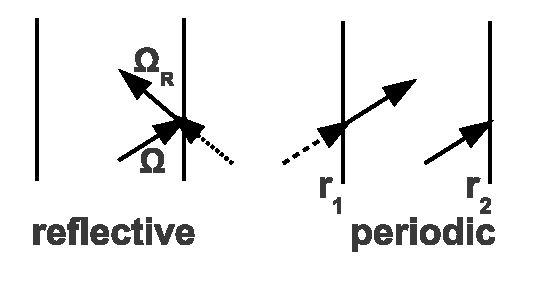
\includegraphics[keepaspectratio, width = 2.0 in]{images/reflectiveperiodic}
    \caption{Reflective and periodic boundary conditions.}
    \label{fig:reflectiveperiodic}
\end{figure}

The final boundary condition we mention is the \textit{white boundary condition}, a condition where all neutrons incident on a boundary reflect back isotropically in angle.  For this case,
\begin{equation}
\begin{split}
 \psi(\mathbf{r}_s,\mathbf{\Omega},E,t) &= \frac{ \int_{\mathbf{\hat{n}} \cdot \mathbf{\Omega}' > 0}   \mathbf{\hat{n}} \cdot \mathbf{\Omega}' \psi (\mathbf{r},\mathbf{\Omega}',E,t)d\Omega' } {  \int_{\mathbf{\hat{n}} \cdot \mathbf{\Omega}' > 0}  \mathbf{\hat{n}} \cdot \mathbf{\Omega}'  d\Omega'    }  \\
             &= \frac{ J_+ (\mathbf{r}_s,E,t) } {  \int_{\mathbf{\hat{n}} \cdot \mathbf{\Omega}' > 0}  \mathbf{\hat{n}} \cdot \mathbf{\Omega}'  d\Omega'    }\, , \, \, \, \,  \, \, \, \mathbf{\hat{n}} \cdot \mathbf{\Omega}' < 0 \, .
\end{split}
\end{equation}
Note the conditions on $\mathbf{\Omega}$ and $\mathbf{\Omega}'$.  The first corresponds to the left hand side and is limited to $\mathbf{\hat{n}} \cdot \mathbf{\Omega}' < 0$, i.e. incoming directions.  Contrarily, $\mathbf{\Omega}'$ is the dummy variable on the right hand side, and is always integrated over the domain where $\mathbf{\hat{n}} \cdot \mathbf{\Omega}' > 0$, i.e. outgoing directions.  This is so because we integrate the entire outgoing neutron population (which is proportional to the outgoing partial current) and then redistribute that number uniformly over all incident directions, i.e. isotropically.

White boundary conditions have had use in lattice physics where an isotropic angular distribution is sometimes relatively accurate.  In particular, the white boundary condition provides a useful fix for reflective conditions in Wigner-Seitz cells, which convert square pin cells into equivalent cylindrical cells, since cylindrical cells can be treated with 1-d methods.  However, while in square cells the reflective conditions work fine, they do not work well in cylindrical geometries (see Figure \ref{fig:wignerseitz}), since neutrons entering at certain angles can spend too much time in the moderator before colliding.  This consequently leads to overprediction of the moderator flux, an artifact known as the Newmarch effect. As a result, white conditions are used.


\begin{figure}[h] 
    \centering
    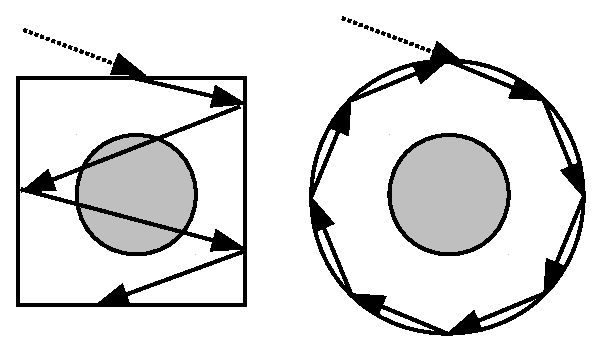
\includegraphics[keepaspectratio, width = 3.0 in]{images/wignerseitz}
    \caption{Square pin cell and equivalent Wigner-Seitz cell.  Same incident direction and location.}
    \label{fig:wignerseitz}
\end{figure}

\section*{Other Transport Equations}

We finish this lecture by presenting in brief two other important transport equations.

\subsection*{Photon Transport}

Photon transport is fundamental to radiation hydrodynamics (an integral aspect of ``bomb'' physics) and astrophysics.  Photon transport can largely be divided into two classes of problems: \textit{radiative transfer}, which consists of the propogation of soft (low energy) x-rays, and \textit{high energy} photon transport, which can largely be treated as we do neutrons.  We briefly describe the former.

The quantity of interest is the intensity, essentially an ``energy angular flux'', and is defined
\begin{equation}
 I_{\nu}(\mathbf{r},\mathbf{\Omega},t) = (h\nu)cn(\mathbf{r},\mathbf{\Omega},E,t) \, ,
\end{equation}
where $h\nu$ is the photon energy.  The ``radiative transfer equation'' is
\begin{equation}
 \frac{1}{c}\frac{\partial I_{\nu}}{\partial t} + \Omega \cdot \nabla I_{\nu} = \rho(\varepsilon_{\nu} - \kappa_{\nu}I_{\nu}) \, ,
 \label{eq:radiative}
\end{equation}
where $\varepsilon$ is a mass emission coefficient (a source term), and $\kappa$ is a mass attenuation coefficient (a loss term).  The radiative transfer equations are nonlinear due to the temperature-dependence of the underlying interaction coefficients (the ``cross-sections), particularly the emission term (which is not explicitly represented in Eq. \ref{eq:radiative}).

For the case of local thermodynamic equilibrium (LTE), Eq. \ref{eq:radiative} is simplified somewhat.  Local thermodynamic equilibrium exists when the quantity $S_{\nu} = \varepsilon_{\nu}/\kappa_{\nu} = B_{\nu}$, where $B_{\nu}$ is the Planck distribution (i.e. the black body spectrum).  In this case, Eq. \ref{eq:radiative} takes the form
\begin{equation}
 \frac{1}{c}\frac{\partial I_{\nu}}{\partial t} + \Omega \cdot \nabla I_{\nu} = \rho \kappa_{\nu} (B_{\nu} - I_{\nu}) \, .
 \label{eq:radiativelte}
\end{equation}

Radiative transfer is inherently a frequency-dependent process: the coefficients depend on the frequency, and a medium emits photons of a wide range of frequencies.  A frequently used approximation is to neglect this dependence in what is called the \textit{grey approximation}, similar to the one-speed studies in neutron transport we will study in the next several lectures.  ``Black bodies'' are also often used; these are pure absorbers whose emission spectrum is the Planck distribution.

To determine the temperature (dependence on which is implicit in all the quantities of Eq. \ref{eq:radiative}), an energy conservation equation is used.  As an example, using the grey approximation and assuming temperature- and spatially-independent coefficients, Eq. \ref{eq:radiative} becomes
\begin{equation}
 \frac{1}{c}\frac{\partial I}{\partial t} + \Omega \cdot \nabla I(\mathbf{r},\mathbf{\Omega},t) = \rho \kappa (acT^4(\mathbf{r},t)- I) \, ,
 \label{eq:radiativegrey}
\end{equation}
where $a$ is the emissivity (as in the Stefan-Boltzmann law) and $T$ is the temperature.  The corresponding energy conservation equation is
\begin{equation}
 \overbrace{c_v \frac{\partial T}{\partial t}}^{\text{energy rate of change}} = \overbrace{\rho \kappa}^{\text{abs. coef.}} \overbrace{\int_{4\pi} I(\mathbf{r},\mathbf{\Omega},t) d\Omega}^{\text{energy flux}} - \overbrace{\rho \kappa a c T^4(\mathbf{r},t)}^{\text{loss due to emission}} + \overbrace{Q(\mathbf{r},t)}^{\text{gains from outside}} \, ,
\end{equation}
where $c_v$ is the specific heat and $Q$ represents any external energy source.


\subsection*{Plasma Transport}

Another area of interest for nuclear engineers is plasma physics.  Let us apply Eq. \ref{eq:generalte} to electrons in a plasma, where we substitute in the Lorentz force for $\mathbf{F}$:
\begin{equation}
  \frac{\partial n}{\partial t} 
   + \mathbf{v} \cdot \nabla n + \frac{e}{m} \Big ( \mathbf{E}+(\mathbf{v}\times \mathbf{B} ) \Big ) \cdot \nabla_{\mathbf{v}} n =   \Big( \frac{\partial n}{\partial t} \Big )_{\mathrm{coll}} +  s \, .
\end{equation}
If we neglect sources and collisions, we arrive at the Vlasov equation:
\begin{equation}
  \frac{\partial n}{\partial t} 
   + \mathbf{v} \cdot \nabla n + \frac{e}{m} \Big ( \mathbf{E}+(\mathbf{v}\times \mathbf{B} ) \Big ) \cdot \nabla_{\mathbf{v}} n =  0 \, .
\end{equation}
Augmented with Maxwell's equations, the Vlasov equation gives a rather complete description of collisionless plasmas.  



\section*{Further Reading}
This lecture follows quite closely the treatment of transport theory in Chapter 1 of Duderstadt and Martin \cite{duderstadt1976tt}.  The reader is encouraged to read that chapter (uploaded to Stellar) and others (MIT libraries should have a copy for the eager beaver).  Bell and Glasstone \cite{bell1970nrt} give a more traditional derivation, as do Duderstadt and Hamilton \cite{duderstadt1976nra}.
 
The treatment of boundary conditions is rather straightforward, but the student may wish to consult e.g. Duderstadt and Martin \cite{duderstadt1976tt} or Lewis and Miller \cite{lewis1993cmn}.  The discussion of white boundary conditions and the Wigner-Seitz dilemma follows that of H\'{e}bert \cite{hebert2009arp}, and the Newmarch effect is identified by Stamm'ler and Abbate \cite{stammler1983mss}.   

The discussion of photon and plasma transport largely follows that of Duderstadt and Martin \cite{duderstadt1976tt}.  The example grey approximation equations are given in a paper by Miller and Lewis \cite{miller1987nrm}, and there is a wealth of literature on the subject.  For those interested in radiative transfer as it applies to atmospheres, see MIT course 12.815.

\begin{exercises}
 
  \item \textbf{Variable Transformations}. 
        Prove the relations given in Eq. \ref{eq:densityrelations}.

%   \item In Lecture \ref{lec:criticality}, the eigenvalue problem, i.e. a problem without an external source, was introduced in operator form.  You probably also know the eigenvalue diffusion equation from reactor physics. 
%   \begin{enumerate}[(a)]
%    \item Write down the 1-d, one group transport equation for an eigenvalue problem in slab geometry (you need to determine the fission source term)
%    \item Assuming isotropic scattering, and an infinite homogeneous, derive a simple expression for $k$ in terms of the cross-sections; what does this expression represent?
%   \end{enumerate}

  \item \textbf{Duderstadt \& Hamilton 4-3}. Suppose that the angular neutron 
        density is given by 
        \begin{equation*}
          n(\mathbf{r},\hat{\bm{\Omega}}) = \frac{n_0}{4\pi} (1-\cos\theta) \, ,
        \end{equation*}
        where $\theta$ is the angle between $\hat{\bm{\Omega}}$ and the 
        $z$-axis. If $A$ is the area perpendicular to the $z$-axis, then 
        what is the number of neutrons passing through the area 
        per second
        \begin{enumerate}[(a)]
         \item per unit solid angle at an angle of 45$^{\text{o}}$ with 
               the $z$-axis
         \item from the negative $z$ to the positive $z$ direction
         \item net 
         \item total?
        \end{enumerate}

  \item \textbf{Duderstadt \& Hamilton 4-4}. In a spherical thermal reactor of 
        radius $R$, it is found that the angular flux can be roughly 
        described by 
        \begin{equation*}
         \psi(\mathbf{r}, E, \hat{\bm{\Omega}}) 
          = \frac{\phi_0}{4\pi} E \exp \left ( -\frac{E}{kT} \right ) \frac{\sin(\pi r/R)}{r} \, .
        \end{equation*}
        Compute the total number of neutrons in the core.

  \item \textbf{Duderstadt \& Hamilton 4-5}. Demonstrate that in an 
        isotropic flux, the partial current density in any direction is
        given by $J_+ = \phi / 4$.


\end{exercises}
